%% For double-blind review submission
% \documentclass[sigplan,review,anonymous]{acmart}
%% For single-blind review submission
%\documentclass[sigplan,review]{acmart}
%% For proofreading
% \documentclass[sigplan,authordraft]{acmart}
%% For final camera-ready submission
\documentclass[10pt,acmtog]{acmart}
%% For booklet
% \documentclass[acmsmall]{acmart}

% !TEX root=../main.tex


%% Basics %%%%%%%%%%%%%%%%%%%%%%%%%%%%%%%%%%%%%%%%%%%%%%%%%%%%%%%%%%%%%%%%%%%%%%

%% Fixes %%

\usepackage{underscore}


%% Fonts %%

\usepackage[utf8]{inputenc}
\usepackage[T1]{fontenc}

\usepackage{stmaryrd}

% \usepackage{tgpagella}
% \usepackage{lucidabr}
\usepackage{libertine}
\usepackage[varqu]{zi4}
\usepackage[libertine]{newtxmath}


%% Programming %%

\usepackage{ifthen}


%% Layout %%

% \usepackage[final]{microtype}


%% Additions %%%%%%%%%%%%%%%%%%%%%%%%%%%%%%%%%%%%%%%%%%%%%%%%%%%%%%%%%%%%%%%%%%%

%% Textual %%

\usepackage{paralist}
\usepackage{quoting}


%% Maths %%

\usepackage{amsmath}
\usepackage{mathpartir}


%% Graphics %%

\usepackage{graphicx}
% \usepackage{xcolor}


%% Tabulations %%

\usepackage{booktabs}
\usepackage{array}


%% Listings %%

% \usepackage[final]{listings}


%% References %%

\usepackage{cleveref}

% !TEX root=../main.tex


%% Fixes %%

\frenchspacing

%% NOTE: uses the same lengths as in `tufte-common.def` and `article.cls`...
\setlength{\bigskipamount}   {3.25ex plus .2ex} %% ...before (sub)section
\setlength{\medskipamount}   {2.3ex  plus .2ex} %% ...after section
\setlength{\smallskipamount} {1.5ex  plus .2ex} %% ...after subsection


%% Numbering %%

% \setcounter{secnumdepth}{2}


%% Compact lists %%
%% NOTE: requires `paralist`

\setlength{\pltopsep}{\smallskipamount}
\setlength{\plpartopsep}{\parskip}
\setlength{\plitemsep}{\parskip}
\setlength{\plparsep}{\parskip}

% !TEX root=../main.tex


%% Helpers %%%%%%%%%%%%%%%%%%%%%%%%%%%%%%%%%%%%%%%%%%%%%%%%%%%%%%%%%%%%%%%%%%%%%

\let\newoperator\DeclareMathOperator


%% Text %%%%%%%%%%%%%%%%%%%%%%%%%%%%%%%%%%%%%%%%%%%%%%%%%%%%%%%%%%%%%%%%%%%%%%%%

\newcommand*{\alert}[1]
  {\textbf{#1}}
\newcommand*{\enquote}[1]
  {``#1''}
\newcommand*{\todo}[1]
  {\ensuremath{\star}\marginnote{\ensuremath{\star}#1}}


%% Lists %%
%% NOTE: requires `paralist`

%% Use compact lists by default
\renewenvironment{itemize}
  {\begin{compactitem}}
  {\end{compactitem}}
\renewenvironment{enumerate}
  {\begin{compactenum}}
  {\end{compactenum}}
\renewenvironment{description}
  {\begin{compactdesc}}
  {\end{compactdesc}}
%% Define starred versions as in-paragraph-lists
\newenvironment{itemize*}
  {\begin{inparitem}}
  {\end{inparitem}}
\newenvironment{enumerate*}
  {\begin{inparenum}}
  {\end{inparenum}}
\newenvironment{description*}
  {\begin{inpardesc}}
  {\end{inpardesc}}


%% Blocks %%

\newenvironment{block}
  {\smallskip}
  {\smallskip}


%% Column types %%
%% NOTE: requires `array`

\newcolumntype{L}{>{$}l<{$}}
\newcolumntype{C}{>{$}c<{$}}
\newcolumntype{R}{>{$}r<{$}}
\newcolumntype{T}{>{\ttfamily}l}
\newcolumntype{S}{>{\sffamily}l}


%% References %%
%% NOTE: requires `cleveref`

\let\see\cref
\let\See\Cref
\let\at\cpageref


%% Citations %%
%% NOTE: requires `natbib`

\let\cite\citep
\let\textcite\citet


%% Math %%%%%%%%%%%%%%%%%%%%%%%%%%%%%%%%%%%%%%%%%%%%%%%%%%%%%%%%%%%%%%%%%%%%%%%%

%% NOTE: change this to \emptyset when using a font that includes a nice standard emptyset
\let\nothing\varnothing


%% Braces %%

\let\<\langle
\let\>\rangle

\newcommand*{\llbrace}
  {\{\!|}
\newcommand*{\rrbrace}
  {|\!\}}


%% Operators %%

\let\lt<
\let\gt>
\let\eq\equiv

\newcommand*{\pp}
  {+\!\!+}


%% Shortcuts %%

\newcommand*{\powerset}
  {\mathcal{P}}

\newcommand*{\NN}{\mathbb{N}}
\newcommand*{\ZZ}{\mathbb{Z}}
\newcommand*{\RR}{\mathbb{R}}
\newcommand*{\CC}{\mathbb{C}}

\newcommand*{\LL}{\mathbb{L}}
\newcommand*{\UU}{\mathbb{U}}
\newcommand*{\BB}{\mathbb{B}}
\renewcommand*{\SS}{\mathbb{S}}

\newoperator{\downto}
  {\;\rightarrow\!\shortmid\;}

\let\to\rightarrow
\let\implies\Rightarrow
\let\infers\vdash

% !TEX root=../main.tex


%% Styles %%%%%%%%%%%%%%%%%%%%%%%%%%%%%%%%%%%%%%%%%%%%%%%%%%%%%%%%%%%%%%%%%%%%%%

\lstdefinestyle{natural}
  {columns=fullflexible
  ,gobble=2
  ,breaklines=true
  ,breakatwhitespace=true
  ,literate=
    %{.}{{$\cdot$}}1
    %{.}{{\ }}1
    {<<}{{$\<$}}1
    {>>}{{$\>$}}1
    {->}{{$\to$\ }}2
    % {--}{{--}}1
    %{_}{{\ }}1
    %{\ "}{{\ \textquotedblleft}}2
    %{"\ }{{\textquotedblright\ }}2
  ,basicstyle={\sffamily}
  ,keywordstyle=[1]{\bfseries}
  ,keywordstyle=[2]{\scshape}
  ,keywordstyle=[3]{}
  %,commentstyle={\itshape}
  %,identifierstyle={\itshape}
  ,emphstyle={\itshape}
  %,stringstyle={\rmfamily}
  ,showstringspaces=false
  ,texcl=true
  ,mathescape=true
  %,escapechar=\$
  %,escapeinside={\{\}}
  ,xleftmargin=1\parindent
  }

\lstdefinestyle{flexible}
  {columns=flexible
  ,gobble=2
  ,fontadjust=true
  ,basicstyle={\ttfamily\small}
  ,commentstyle={\itshape}
  ,keywordstyle={\bfseries}
  %,identifierstyle={\itshape}
  %,stringstyle={\ttfamily}
  ,emphstyle={\itshape}
  ,showstringspaces=false
  ,texcl=true
  ,mathescape=true
  %,escapechar=\$
  %,escapeinside={\{\}}
  ,xleftmargin=1\parindent
  }

\lstdefinestyle{literate}
  {literate=
    {\\}{{$\lambda$}}1
    {\\\$}{{\$}}1 %NOTE: otherwise eaten by `\`, NOTE: prevents \$ to be parsed as math escape
    {\\/}{{$\vee$}}1
    {/\\}{{$\wedge$}}1
    {A.}{{$\forall$}}1
    {E.}{{$\exist$}}1
    {->}{{$\rightarrow$ }}1
    {<-}{{$\leftarrow$}}1
    {<=}{{$\leq$}}1
    {>=}{{$\geq$}}1
    {>>=}{{>>=}}3 %NOTE: otherwise eaten by `>=`
    {\{|}{{$\{\!|\!$}}1
    {|\}}{{$\!|\!\}$}}1
    {\{|*|\}}{{$\{\!|\!\!\star\!\!|\!\}$}}3
  }


%% Definitions %%%%%%%%%%%%%%%%%%%%%%%%%%%%%%%%%%%%%%%%%%%%%%%%%%%%%%%%%%%%%%%%%

%% Tasks %%

\lstdefinelanguage{tasks}
  {sensitive=true
  ,morekeywords=[1]{if,then,else,case,of}
  ,morekeywords=[2]{Bool,Int,String,Store,List}
  ,morestring=[b]"
  ,morecomment=[l]--
  ,morecomment=[n]{\{-}{-\}}
  }[keywords,strings,comments]
\lstdefinestyle{tasks}
  {style=natural
  ,literate=
    {\\}{{$\lambda$}}1
    {>>=}{{$\Then$\ }}1
    {>>?}{{$\Next$\ }}1
    {<&>}{{$\And$\ }}1
    {<|>}{{$\Or$\ }}1
    {<?>}{{$\Xor$\ }}1
    {edit}{{$\Edit$}}1
    {enter}{{$\Enter$}}1
    {store}{{$\Change$}}1
    {fail}{{$\Fail$}}1
    {==}{{$\equiv$\ }}1
    {/=}{{$\nequiv$\ }}1
  }

\lstnewenvironment{TASK}[1][]
  {\lstset{language=tasks,style=tasks,#1}}
  {}
\newmacro{TS}[1][1]
  {\lstinline[language=tasks,style=tasks,#1]}
\newmacro{includeTASK}[2][]
  {\lstinputlisting[language=tasks,style=tasks,#1]{#2}}


%% Flows %%

\lstdefinelanguage{flows}
  {sensitive=true
  ,morekeywords=[1]{module,where,define,using,as,yielding,share,holding,with,do,for,fork,then,when,next,done,on,and,or,not,readonly,writeonly,readwrite}
  ,morekeywords=[2]{Bool,Int,String,Shared,List, Date,Document,Photo, Citizen,Company,Declaration}
  ,morekeywords=[3]{True,False,Just,Nothing,List}
  ,morestring=[b]"
  ,morecomment=[l]--
  ,morecomment=[n]{\{-}{-\}}
  }[keywords,strings,comments]

% \lstMakeShortInline[language=flows,style=natural] | % |
\lstnewenvironment{FLOW}[1][]
  {\lstset{language=flows,style=natural,#1}}
  {}
\newmacro{FL}[1][1]
  {\lstinline[language=flows,style=natural,#1]}
\newmacro{includeFLOW}[2][]
  {\lstinputlisting[language=flows,style=natural,#1]{#2}}


%% Clean %%

\lstdefinelanguage{clean}
  {sensitive=true
  %,alsoletter={ABCDEFGHIJKLMNOPQRSTUVWXYZabcdefghijklmnopqrstuvwxyz_`}
  %,alsoletter={~!@\#$\%^\&*-+=?<>:|\\} %$
  ,morekeywords={from,definition,implementation,import,module,system,code,inline,if,case,of,let,let!,in,where,with,class,instance,generic,derive,dynamic,infix,infixl,infixr}
  ,morestring=[b]"
  ,morestring=[b]'
  ,morecomment=[l]//
  ,morecomment=[n]{/*}{*/}
  }[keywords,strings,comments]

\lstnewenvironment{CLEAN}[1][]
  {\lstset{language=clean,style=flexible,#1}}
  {}
\newmacro{CL}[1][1]
  {\lstinline[language=clean,style=flexible,#1]}
\newmacro{includeCLEAN}[2][1]
  {\lstinputlisting[language=clean,style=flexible,#1]{#2}}


\newlogo[ITASKS]{iTasks}
\newlogo{BPMN}
\newlogo{BPEL}
\newlogo{UML}
\newlogo{WFN}

\newlogo{EDSL}
\newlogo{GUI}

\newlogo{STW}
\newlogo{NWO}

% !TEX root=../main.tex



%% Host language %%%%%%%%%%%%%%%%%%%%%%%%%%%%%%%%%%%%%%%%%%%%%%%%%%%%%%%%%%%%%%%


\newkeyword[IF]  {if}
\newkeyword[THEN]{then}
\newkeyword[ELSE]{else}

\newkeyword[Let]{let}
\newkeyword[In]{in}

\newkeyword[Ref] {ref}


\newmacro{If}[3]
  {\IF #1 \THEN #2 \ELSE #3}



%% Values %%


\newmathcommand{unit}{\<\>}


\newvalue{True}
\newvalue{False}
\newvalue[Not]{not}


\newmacro{str}[1]
  {\text{``#1''}}

\newoperator{Length}{\mathrm{length}}


\newvalue[Map]{map}
\newvalue[Fst]{fst}
\newvalue[Snd]{snd}
\newvalue[Assoc]{assoc}



%% Types %%


\newtype{Unit}
\newtype{Bool}
\newtype{Nat}
\newtype{Int}
\newtype{String}
\newtype[Reference]{Ref}
\newtype{Task}
\newtype{Maybe}

\newtype{Euro}



%% Object language %%%%%%%%%%%%%%%%%%%%%%%%%%%%%%%%%%%%%%%%%%%%%%%%%%%%%%%%%%%%%


\let\And\relax
\newoperator{Then}  {\blacktriangleright}
\newoperator{Next}  {\vartriangleright}
\newoperator{And}   {\Join}
\newoperator{Or}    {\blacklozenge}
\newoperator{Xor}   {\lozenge}
\newoperator{Edit}  {\square}
\newoperator{View}  {\overline{\square}}
\newoperator{Enter} {\boxtimes}
\newoperator{Update}{\blacksquare}
\newoperator{Watch} {\overline{\blacksquare}}
\newoperator{Fail}  {\lightning}

\newoperator{AndOr} {\DEPRECATED}



%% Events %%


\newvalue[Left]   {L}
\newvalue[Right]  {R}


\newvalue[Clear]   {C}
\newvalue[Continue]{N}
\newvalue[Pick]    {P}


\newvalue[First]  {F}
\newvalue[Second] {S}
\newvalue[Here]   {H}



%% Semantic functions %%%%%%%%%%%%%%%%%%%%%%%%%%%%%%%%%%%%%%%%%%%%%%%%%%%%%%%%%%


\newmathcommand{evaluate}[rel]
  {\;\downarrow\;}
\newmathcommand{normalise}[rel]
  % {\;\rightarrow\!\shortmid\;}
  {\;\Downarrow\;}
\newmacro{handle}[1]
  {\mathrel{\;\xrightarrow{\;#1\;}\;}}
\newmacro{drive}[1]
  {\mathrel{\;\xRightarrow{\;#1\;}\;}}


\newmathcommand{Value}[cal]
  {V}
\newmathcommand{Firsts}[cal]
  {F}
\newmathcommand{Interface}[cal]
  {U}
\newmathcommand{Succeeding}[cal]
  {S}



%% Depricated %%%%%%%%%%%%%%%%%%%%%%%%%%%%%%%%%%%%%%%%%%%%%%%%%%%%%%%%%%%%%%%%%%

\newvalue[Execute] {<depricated>}

% !TEX root=pldi2019.tex


%% Helpers %%%%%%%%%%%%%%%%%%%%%%%%%%%%%%%%%%%%%%%%%%%%%%%%%%%%%%%%%%%%%%%%%%%%%

\newmacro{newrule}[4][2]
  {\newmacro{#1}{\inferrule*[lab={#1},right={$#2$}]
    {#3}
    {#4}}}
\newmacro{userule}
  {\usemacro}
\newmacro{refrule}[1]
  {\ifthenelse{\isundefined{#1}}
    {\GenericError{}{Rule `#1` is not defined}{}{}}
    {\textsc{#1}}}


\newif\ifstateful
\statefulfalse
\newmacro{st}[2][1]
  {\ifthenelse{\isempty{#1}}
    {\ifstateful{,\:s#2}\else{}\fi}
    {\ifstateful{,\:[#1]s#2}\else{}\fi}}
\newmacro{St}[1]
  {\ifstateful{,\:\Sigma#1}\else{}\fi}



%% Typing %%%%%%%%%%%%%%%%%%%%%%%%%%%%%%%%%%%%%%%%%%%%%%%%%%%%%%%%%%%%%%%%%%%%%%


\newmacro{RelationT}
  {\Gamma,\Sigma \infers e : \tau}


\newrule{T-Var}
  {x:\tau\in\Gamma}
  {\Gamma,\Sigma\infers x:\tau}


\newrule{T-Abs}
  {\Gamma[x:\tau_1] ,\Sigma \infers e:\tau_2}
  {\Gamma,\Sigma \infers \lambda x : \tau_1 . e :\tau_1 \to \tau_2}

\newrule{T-App}
  {\Gamma,\Sigma \infers e_1:\tau_1\to\tau_2\\
   \Gamma,\Sigma \infers e_2:\tau_1}
  {\Gamma,\Sigma \infers e_1 e_2 :\tau_2}


\newrule{T-If}
  {\Gamma,\Sigma \infers e_1:\Bool\\
   \Gamma,\Sigma \infers e_2:\tau\\
   \Gamma,\Sigma \infers e_3:\tau}
  {\Gamma,\Sigma \infers \If{e_1}{e_2}{e_3}:\tau}


\newrule{T-Pair}
    {\Gamma,\Sigma \infers e_1 : \tau_1 \\
     \Gamma,\Sigma \infers e_2 : \tau_2}
    {\Gamma,\Sigma \infers \tuple{e_1, e_2} :\tau_1 \times \tau_2}


\newrule{T-Ref}
  {\Gamma,\Sigma \infers e:\tau}
  {\Gamma,\Sigma \infers \Ref e :\Reference \tau}

\newrule{T-Deref}
  {\Gamma,\Sigma \infers e:\Reference \tau}
  {\Gamma,\Sigma\infers\ !e:\tau}

\newrule{T-Assign}
  {\Gamma,\Sigma\infers e_1:\Reference \tau\\
   \Gamma,\Sigma\infers e_2:\tau}
  {\Gamma,\Sigma\infers e_1 := e_2:\Unit}

\newrule{T-Loc}
  {\Sigma(l) = \tau}
  {\Gamma,\Sigma\infers l:\Reference \tau}


\newrule{T-Edit}
  {\Gamma,\Sigma \infers e : \tau}
  {\Gamma,\Sigma \infers \Edit e : \Task \tau}

\newrule{T-Fill}
  {\ }
  {\Gamma,\Sigma \infers \Enter \tau : \Task \tau}

\newrule{T-Update}
  {\Gamma,\Sigma \infers e : \Reference \tau}
  {\Gamma,\Sigma \infers \Update e : \Task \tau}


\newrule{T-Fail}
  {\ }
  {\Gamma,\Sigma \infers \Fail : \Task \tau}


\newrule{T-Then}
  {\Gamma,\Sigma \infers e_1 : \Task \tau_1 \\
   \Gamma,\Sigma \infers e_2 : \tau_1 \to \Task \tau_2}
  {\Gamma,\Sigma \infers e_1 \Then e_2 : \Task \tau_2}


\newrule{T-Next}
  {\Gamma,\Sigma \infers e_1 : \Task \tau_1 \\
   \Gamma,\Sigma \infers e_2 : \tau_1 \to \Task \tau_2}
  {\Gamma,\Sigma \infers e_1 \Next e_2 : \Task \tau_2}


\newrule{T-And}
  {\Gamma,\Sigma \infers e_1 : \Task \tau_1 \\
   \Gamma,\Sigma \infers e_2 : \Task \tau_2}
  {\Gamma,\Sigma \infers e_1 \And e_2 : \Task\,(\tau_1 \times \tau_2)}


\newrule{T-Or}
  {\Gamma,\Sigma \infers e_1 : \Task \tau \\
   \Gamma,\Sigma \infers e_2 : \Task \tau }
  {\Gamma,\Sigma \infers e_1 \Or e_2 : \Task \tau}


\newrule{T-Xor}
  {\Gamma,\Sigma \infers e_1 : \Task \tau \\
   \Gamma,\Sigma \infers e_2 : \Task \tau }
  {\Gamma,\Sigma \infers e_1 \Xor e_2 : \Task \tau}


\newrule{T-Appoint}
  {\Gamma,\Sigma\infers e:\Task\tau}
  {\Gamma,\Sigma\infers u \At e:\Task\tau}



%% Evaluation %%%%%%%%%%%%%%%%%%%%%%%%%%%%%%%%%%%%%%%%%%%%%%%%%%%%%%%%%%%%%%%%%%


\newmacro{RelationE}
  {e,s \evaluate v,s'}


\newrule{E-Value}[v\in\set{\lambda x:\tau.e, \unit, l, B, I, S}]
  {\ }
  {v,s\evaluate v,s}

\newrule{E-App}
  {e_1,s\evaluate \lambda x:\tau.e_1',s'\\
   e_2,s'\evaluate v_2,s''\\
   e_1'[x\mapsto v_2],s''\evaluate v_1,s'''}
  {e_1 e_2,s \evaluate v_1,s'''}


\newrule{E-IfTrue}
    {e_1,s\evaluate \True,s'\\
     e_2,s'\evaluate v,s''}
    {\If{e_1}{e_2}{e_3},s\evaluate v,s''}

\newrule{E-IfFalse}
  {e_1,s\evaluate \False,s'\\
   e_3,s'\evaluate v,s''}
  {\If{e_1}{e_2}{e_3},s\evaluate v,s''}


\newrule{E-Pair}
  {e_1,s\evaluate v_1,s'\\
   e_2,s'\evaluate v_2,s''}
  {\tuple{e_1,e_2},s\evaluate\tuple{v_1,v_2},s''}


\newrule{E-Ref}
  {e,s\evaluate v,s'\\
   l\not\in Dom(s)}
  {\Ref e,s\evaluate l,s'[l\mapsto v]}

\newrule{E-Deref}
  {e,s\evaluate l,s'}
  {!e,s\evaluate s'(l),s'}

\newrule{E-Assign}
  {e_1,s\evaluate l,s'\\
   e_2,s'\evaluate v_2,s''}
  {e_1:=e_2,s\evaluate \unit,s''[l\mapsto v_2]}


\newrule{E-Sequence}
  {?}
  {e_1;e_2 \evaluate ?}

\newrule{E-Edit}
  {e,s \evaluate v,s'}
  {\Edit e , s\evaluate \Edit v,s'}

\newrule{E-Fill}
  {\ }
  {\Enter \tau,s \evaluate \Enter \tau,s}

\newrule{E-Update}
  {e,s\evaluate l,s'}
  {\Update e ,s\evaluate \Update l,s'}


\newrule{E-Fail}
  {\ }
  {\Fail,s \evaluate \Fail,s}


\newrule{E-Then}
  {e_1 ,s\evaluate t_1,s'}
  {e_1 \Then e_2,s \evaluate t_1 \Then e_2,s'}

\newrule{E-Next}
  {e_1 ,s\evaluate t_1,s'}
  {e_1 \Next e_2 ,s\evaluate t_1 \Next e_2,s'}


\newrule{E-And}
  {e_1 ,s\evaluate t_1 ,s'\\
   e_2 ,s'\evaluate t_2,s''}
  {e_1 \And e_2 ,s\evaluate t_1 \And t_2,s''}


\newrule{E-Or}
  {e_1 ,s\evaluate t_1 ,s'\\
   e_2 ,s'\evaluate t_2,s''}
  {e_1 \Or e_2 ,s\evaluate t_1 \Or t_2,s''}

\newrule{E-Xor}
  {\ }
  {e_1 \Xor e_2 ,s\evaluate e_1 \Xor e_2,s}


\newrule{E-Appoint}
    {e,s\evaluate t,s'}
    {u \At e,s\evaluate u \At t,s'}



%% Normalisation %%%%%%%%%%%%%%%%%%%%%%%%%%%%%%%%%%%%%%%%%%%%%%%%%%%%%%%%%%%%%%%


\newmacro{RelationS}
  {t,s \stride t',s'}


\newrule{S-Edit}
  { }
  {\Edit v,s \stride \Edit v,s}

\newrule{S-Fill}
  { }
  {\Enter \tau,s \stride \Enter \tau,s}

\newrule{S-Update}
  { }
  {\Update l,s \stride \Update l,s}


\newrule{S-Fail}
  { }
  {\Fail,s \stride \Fail,s}


\newrule{S-ThenStay}[\Value(t_1',s') = \bot]
  {t_1,s \stride t_1',s'}
  {t_1 \Then e_2,s \stride t_1' \Then e_2,s'}

\newrule{S-ThenFail}[\Value(t_1',s') = v_1 \land \Failing(t_2,s'')]
  {t_1,s \stride t_1',s' \\
   e_2\ v_1,s' \evaluate t_2,s''}
  {t_1 \Then e_2,s \stride t_1' \Then e_2,s'}

\newrule{S-ThenCont}[\Value(t_1',s') = v_1 \land \lnot\Failing(t_2,s'')]
  {t_1,s \stride t_1',s' \\
   e_2\ v_1,s' \evaluate t_2 ,s'' \\
   t_2,s'' \stride t_2',s'''}
  {t_1 \Then e_2,s \stride t_2',s'''}

\newrule{S-Next}
  {t_1,s \stride t_1',s'}
  {t_1 \Next e_2,s \stride t_1' \Next e_2,s'}


\newrule{S-And}
  {t_1,s  \stride t_1',s' \\
   t_2,s' \stride t_2',s''}
  {t_1 \And t_2,s \stride t_1' \And t_2',s''}


\newrule{S-OrLeft}[\Value(t_1',s') = v_1]
  {t_1,s  \stride t_1',s'}
  {t_1 \Or t_2,s \stride t_1',s'}

\newrule{S-OrRight}[\Value(t_1',s') = \bot \land \Value(t_2',s'') = v_2]
  {t_1,s  \stride t_1',s' \\
   t_2,s' \stride t_2',s''}
  {t_1 \Or t_2,s \stride t_2',s''}

\newrule{S-OrNone}[\Value(t_1',s') = \bot \land \Value(t_2',s'') = \bot]
  {t_1,s  \stride t_1',s' \\
   t_2,s' \stride t_2',s''}
  {t_1 \Or t_2,s \stride t_1' \Or t_2',s''}


\newrule{S-Xor}
  { }
  {e_1 \Xor e_2,s \stride e_1 \Xor e_2,s}

\newrule{S-Eval}[e \neq e']
    {e,s \evaluate e',s' \\
     e',s' \stride e'',s''}
    {e,s \stride e'',s''}


\newrule{S-Appoint}
  {t,s\stride t',s'}
  {u \At t,s\stride u \At t',s'}


% \newrule{S-Next}[t_1' = \Edit v]
%   {t_1,\Sigma \stride t_1'\st{'}   \\
%    e\ v \evaluate t_2       \\
%    t_2\st{'} \stride t_2'\st{''} }
%   {t_1 \Next e,\Sigma \stride t_2'\st{''}}

% \newrule{S-NextEval}
%   {e_1,\Sigma \stride u_1\st{'}}
%   {e_1 \Next e_2,\Sigma \stride u_1 \Next e_2\st{'}}




%% Normalisation %%


\newmacro{RelationN}
  {e,s \normalise t,s'}


\newrule{N-Done}[\Dirty(s,s'') \cap \Watching(t') = \nothing]
    {e,s \evaluate t,s' \\
     t,s' \stride t',s''}
    {t,s \normalise t',s''}


\newrule{N-Stride}[\Dirty(s,s'') \cap \Watching(t') \neq \nothing]
    {e,s \evaluate t,s' \\
     t,s' \stride t',s'' \\
     t',s'' \normalise t'',s'''}
    {e,s \normalise t'',s''}



%% Handling %%


\newmacro{RelationH}
  {t,s \handle{i} t',s'}

\newrule{H-Change}[v, v' : \tau]
  { }
  {\Edit v,s \handle{v'} \Edit v',s}

\newrule{H-Empty}[v : \tau]
  { }
  {\Edit v,s \handle{\Empty} \Enter \tau,s}

\newrule{H-Fill}[v' : \tau]
  { }
  {\Enter \tau,s \handle{v'} \Edit v',s}

\newrule{H-Update}[s(l), v' : \tau]
  { }
  {\Update l,s \handle{v'} \Update l,s[l \mapsto v']{}}


\newrule{H-PassThen}
  {t_1,s \handle{i} t_1',s'}
  {t_1 \Then e_2,s \handle{i} t_1' \Then e_2,s'}

\newrule{H-PassNext}
  {t_1,s \handle{i} t_1',s'}
  {t_1 \Next e_2,s \handle{i \neq \Continue} t_1' \Next e_2,s'}

\newrule{H-Next}[\Value{(t_1,s)}\equiv v_1 \wedge \neg\Failing{(t_2,s')}]
  {e_2 v_1,s\stride t_2,s'}
  {t_1 \Next e_2,s \handle{\Continue} t_2,s'}


\newrule{H-FirstAnd}
  {t_1,s \handle{i} t_1',s' }
  {t_1 \And t_2,s \handle{\First i} t_1' \And t_2,s'}

\newrule{H-SecondAnd}
  {t_2,s \handle{i} t_2',s'}
  {t_1,s \And t_2 \handle{\Second i} t_1 \And t_2',s'}


\newrule{H-FirstOr}
  {t_1,s \handle{i} t_1',s'}
  {t_1 \Or t_2,s \handle{\First i} t_1' \Or t_2,s'}

\newrule{H-SecondOr}
  {t_2,s \handle{i} t_2',s' }
  {t_1 \Or t_2,s \handle{\Second i} t_1 \Or t_2',s'}


\newrule{H-PickLeft}[e_1,s\evaluate t_1,s'\wedge \neg\Failing(t_1,s')]
  { }
  {e_1 \Xor e_2,s \handle{\Left} e_1,s}

\newrule{H-PickRight}[e_2,s\evaluate t_2,s'\wedge \neg\Failing(t_2,s')]
  { }
  {e_1 \Xor e_2,s \handle{\Right} e_2,s}


\newrule{H-Appoint}
  {t,s \handle{i} t',s'}
  {u \At t,s\handle{i} u \At t',s'}



%%%%


% \newrule{H-Stay'}[\Value(t_1) = \bot]
%   {\ }
%   {t_1 \Next e,\Sigma \handle{\Next} t_1 \Next e,\Sigma}

% \newrule{H-Next'}[\Value(t_1) = v]
%   {e\ v \evaluate t_2    \\
%    t_2,\Sigma \stride t_2'\st{'} }
%   {t_1 \Next e,\Sigma \handle{\Next} t_2'\st{'}}

% \newrule{H-Stay}[\Value(t_1) = \bot]
%   {\ }
%   {t_1 \Then e,\Sigma \handle{\Execute \pi} t_1 \Then e,\Sigma}

% \newrule{H-Fail'}[\Value(t_1) = v \land t_2 = \Fail]
%   {e\ v \evaluate t_2    \\
%    t_2,\Sigma \handle{\Pick \pi} t_2'\st{'} }
%   {t_1 \Then e,\Sigma \handle{\Execute \pi} t_1 \Then e,\Sigma}

% \newrule{H-Next}[\Value(t_1) = v \land t_2 \neq \Fail]
%   {e\ v \evaluate t_2    \\
%    t_2,\Sigma \handle{\Pick \pi} t_2'\st{'} }
%   {t_1 \Then e,\Sigma \handle{\Execute \pi} t_2'\st{'}}

% \newrule{H-PassS}
%   {t_1,\Sigma \handle{i} t_1'\st{'}}
%   {t_1 \Next e,\Sigma \handle{i} t_1' \Next e\st{'}}

% \newrule{H-Pass}[i \neq \Execute \pi]
%   {t_1,\Sigma \handle{i} t_1'\st{'}       \\
%    t_1' \Then e\st{'} \stride t_2\st{''} }
%   {t_1 \Then e,\Sigma \handle{i} t_2\st{''}}

% \newrule{H-Fallback}
%   { }
%   {t,\Sigma \handle{i} t,\Sigma}



%% Driving %%


\newmacro{RelationD}
  {t,s \drive{i} t',s'}


\newrule{D-Handle}
  {t,s \handle{i} t',s' \\
   t',s' \normalise t'',s''}
  {t,s \drive{i} t'',s''}

% !TEX root=pldi2019.tex


%% Language %%%%%%%%%%%%%%%%%%%%%%%%%%%%%%%%%%%%%%%%%%%%%%%%%%%%%%%%%%%%%%%%%%%%

\newmacro{G-Language}{
  \begin{grammar}
    Expressions
      & e    &::= & \lambda x:\tau.\ e   & – abstraction \\
      &      &\mid& e_1\ e_2             & – application \\
      &      &\mid& x                    & – variable \\
      &      &\mid& c                    & – constant \\
    \addlinespace
      &      &\mid& e_1 \star e_2        & – operation \\
      &      &\mid& \If{e_1}{e_2}{e_3}   & – branch \\
      &      &\mid& \tuple{e_1, e_2}     & – pair \\
      &      &\mid& \Fst e               & – first projection \\
      &      &\mid& \Snd e               & – second projection \\
      &      &\mid& \unit                & – unit \\
    \addlinespace
      &      &\mid& \Ref e               & – reference \\
      &      &\mid& !e                   & – dereference \\
      &      &\mid& e_1 := e_2           & – assignment \\
      % &      &\mid& e_1; e_2             & – sequence \\
      &      &\mid& l                    & – location \\
    \addlinespace
      &      &\mid& p                    & – pretask \\
    \addlinespace
    Constants
      & c    &::= & B                    & – boolean \\
      &      &\mid& I                    & – integer \\
      &      &\mid& S                    & – string
  \end{grammar}
}

\newmacro{G-Language-Compact}{
  \begin{grammar*}
    e ::= &                                                     & Expressions \\
    \mid  & \lambda x:\tau.\ e \Mid  e_1\ e_2                   & – abstraction, application \\
    \mid  & x \Mid  c                                           & – variable, constant \\
    \mid  & \If{e_1}{e_2}{e_3} \Mid e_1 \star e_2               & – branch, operation \\
    \mid  & \tuple{e_1, e_2} \Mid \Fst e \Mid \Snd e \Mid \unit & – pair, projections, unit \\
    \mid  & \Ref e \Mid  !e \Mid  e_1 := e_2 \Mid  l            & – references and locations \\
    \mid  & p                                                   & – pretask \\
    c ::= &                                                     & Constants \\
    \mid  & B \Mid  I \Mid  S                                   & – booleans, integers, strings
  \end{grammar*}
}

\newmacro{G-Pretasks}{
  \begin{grammar}
    Pretasks
      & p    &::= & \Edit e              & – valued editor \\
      &      &\mid& \Enter \tau          & – unvalued editor \\
      &      &\mid& \Update e            & – stored editor \\
    \addlinespace
      &      &\mid& e_1 \Then e_2        & – step \\
      &      &\mid& e_1 \Next e_2        & – user step \\
    \addlinespace
      &      &\mid& e_1 \And e_2         & – composition \\
    \addlinespace
      &      &\mid& e_1 \Or e_2          & – choice \\
      &      &\mid& e_1 \Xor e_2         & – user choice \\
    \addlinespace
      &      &\mid& u \At e              & – appoint \\
      &      &\mid& \Fail                & – fail task
  \end{grammar}
}

\newmacro{G-Pretasks-Compact}{
  \begin{grammar*}
    p ::= &                                              & Pretasks \\
    \mid  & \Edit e \Mid   \Enter \tau  \Mid   \Update e & – editors: valued, unvalued, stored \\
    \mid  & e_1 \Then e_2 \Mid   e_1 \Next e_2           & – steps: system, user \\
    \mid  & e_1 \And e_2                                 & – pairing \\
    \mid  & e_1 \Or e_2 \Mid   e_1 \Xor e_2              & – choice: system, user \\
    \mid  & u \At e \Mid   \Fail                         & – appoint, fail
  \end{grammar*}
}

\newmacro{G-Types}{
  \begin{grammar}
    Types
      & \tau &::= & \tau_1 \to \tau_2    & – function type \\
      &      &\mid& \tau_1 \times \tau_2 & – product type \\
      &      &\mid& \Unit                & – unit type \\
      &      &\mid& \Reference \tau      & – reference type \\
      &      &\mid& \Task \tau           & – task type \\
      &      &\mid& \beta                & – basic type \\
      % &      &\mid& \alpha               & – universal type \\
    Basic types
      &\beta &::= & \Bool                & – boolean type \\
      &      &\mid& \Int                 & – integer type \\
      &      &\mid& \String              & – string type \\
  \end{grammar}
}

\newmacro{G-Types-Compact}{
  \begin{grammar*}
    \tau ::=  &                                               & Types \\
    \mid      & \tau_1 \to \tau_2 \Mid   \tau_1 \times \tau_2 & – function type, product type \\
    \mid      & \Unit \Mid   \Reference \tau                  & – unit type, reference type \\
    \mid      & \Task \tau \Mid   \beta                       & – task type, basic type \\
    \beta ::= &                                               & Basic types \\
    \mid      & \Bool \Mid   \Int \Mid   \String              & – boolean, integer, string
  \end{grammar*}
}

\newmacro{G-Values}{
  \begin{grammar}
    Values
      & v    &::= & \lambda x:\tau.\ e   & – abstraction \\
      &      &\mid& \tuple{v_1, v_2}     & – pair value \\
      &      &\mid& \unit                & – unit \\
      &      &\mid& c                    & – constant \\
      &      &\mid& l                    & – location \\
      &      &\mid& t                    & – task \\
    Tasks
      & t    &::= & \Edit v              & – valued editor \\
      &      &\mid& \Enter \tau          & – unvalued editor \\
      &      &\mid& \Update l            & – stored editor \\
      &      &\mid& \Fail                & – fail task \\
      &      &\mid& t_1 \Then e_2        & – step \\
      &      &\mid& t_1 \Next e_2        & – user step \\
      &      &\mid& t_1 \And t_2         & – composition \\
      &      &\mid& t_1 \Or t_2          & – choice \\
      &      &\mid& t_1 \Xor t_2         & – user choice
  \end{grammar}
}

\newmacro{G-Values-Compact}{
  \begin{grammar*}
    v ::= &                                          & Values \\
      \mid& \lambda x:\tau.\ e                       & – abstraction \\
      \mid& \tuple{v_1, v_2} \Mid \unit              & – pair value, unit \\
      \mid& c \Mid l \Mid t                          & – constant, location, task \\
    t ::= &                                          & Tasks \\
      \mid& \Edit v \Mid \Enter \tau \Mid \Update l  & – editor tasks \\
      \mid& \Fail                                    & – fail task \\
      \mid& t_1 \Then e_2 \Mid t_1 \Next e_2         & – steps \\
      \mid& t_1 \And t_2                             & – composition \\
      \mid& t_1 \Or t_2 \Mid e_1 \Xor e_2            & – choices
  \end{grammar*}
}

\newmacro{G-Inputs}{
  \begin{grammar}
    Inputs
      & i    & ::=& a                    & – action \\
      &      &\mid& \First i             & – pass to first \\
      &      &\mid& \Second i            & – pass to second \\
    Actions
      & a    & ::=& v                    & – change editor to value \\
      &      &\mid& \Empty               & – empty an editor \\
      &      &\mid& \Continue            & – continue with next task \\
      &      &\mid& \Pick                & – pick route \\
    Routes
      & r    & ::=& \Left                & – go left \\
      &      &\mid& \Right               & – go right \\
  \end{grammar}
}

\newmacro{G-Inputs-Compact}{
  \begin{grammar*}
    i ::= &                                 & Inputs \\
    \mid  & a \Mid \First i \Mid \Second i  & – action, pass to first or second \\
    a ::= &                                 & Actions \\
    \mid  & v \Mid \Empty                   & – change to value, empty editor \\
    \mid  & \Continue \Mid \Pick r          & – continue, pick route \\
    r ::= &                                 & Routes \\
    \mid  &\Left \Mid \Right                & – go left or right \\
  \end{grammar*}
}

% !TEX root=pldi2019.tex


%% Language %%%%%%%%%%%%%%%%%%%%%%%%%%%%%%%%%%%%%%%%%%%%%%%%%%%%%%%%%%%%%%%%%%%%

\newmacro{O-Value}{
  \begin{flalign*}
    \begin{array}{lcl}
      \multicolumn{3}{l}{\Value : \mathrm{Tasks} \rightharpoonup \mathrm{Values}} \\
      \Value(\Edit v, s)       &=& v \\
      \Value(\Enter \tau, s)   &=& \bot \\
      \Value(\Update l, s)  &=& s(l) \\
      \Value(\Fail, s)         &=& \bot \\
      \Value(t_1 \Then e_2, s) &=& \bot \\
      \Value(t_1 \Next e_2, s) &=& \bot \\
      \Value(t_1 \And t_2, s)  &=& \left\{
        \begin{array}{ll}
          \tuple{v_1, v_2}  & \when\ \Value(t_1, s) = v_1 \land \Value(t_2, s) = v_2 \\
          \bot              & \otherwise
        \end{array}
      \right. \\
      \Value(t_1 \Or t_2, s)   &=& \left\{
        \begin{array}{ll}
          v_1               & \when\ \Value(t_1, s) = v_1 \\
          v_2               & \when\ \Value(t_1, s) = \bot \land \Value(t_2, s) = v_2 \\
          \bot              & \otherwise
        \end{array}
      \right. \\
      \Value(t_1 \Xor t_2, s)  &=& \bot\\
      \Value(u \At t, s)  &=& \Value(t,s)
    \end{array} & &&
  \end{flalign*}
}

\newmacro{O-Inputs}{
  \begin{flalign*}
    \begin{array}{lcl}
      \multicolumn{3}{l}{\Inputs : \mathrm{Tasks} \to \powerset(\mathrm{Inputs})} \\
      \Inputs(\Edit v:\Task\tau)   &=& \set{v':\tau, \Empty} \\
      \Inputs(\Enter \tau)         &=& \set{v':\tau} \\
      \Inputs(\Update l:\Task\tau) &=& \set{v':\tau} \\
      \Inputs(\Fail)               &=& \nothing \\
      \Inputs(t_1 \Then e_2)       &=& \Inputs(t_1) \\
      \Inputs(t_1 \Next e_2)       &=& \Inputs(t_1) \cup \set{\Continue \mid \Value{(t_1)} = v_1 \land \lnot\Failing(e_2 v_1)} \\
      \Inputs(t_1 \And t_2)        &=& \set{\First\ i \mid i \in \Inputs(t_1)} \cup \set{\Second\ i \mid i \in \Inputs(t_2)} \\
      \Inputs(t_1 \Or t_2)         &=& \set{\First\ i \mid i \in \Inputs(t_1)} \cup \set{\Second\ i \mid i \in \Inputs(t_2)} \\
      \Inputs(e_1 \Xor e_2)        &=& \set{\Left, \Right} \\
      \Inputs(u_1 \At t)           &=& \set{u_2 \At i\mid u_2 \At i \in \Inputs(t)} \cup \set{u_1 \At i\mid i\in \Inputs(t)}
    \end{array} & &&
  \end{flalign*}
}

\newmacro{O-Failing}{
  \begin{flalign*}
    \begin{array}{lcl}
      \multicolumn{3}{l}{\Failing : \mathrm{Tasks} \to \mathrm{Booleans}} \\
      \Failing(\Edit v,s)       &=& \False \\
      \Failing(\Enter \tau,s)   &=& \False \\
      \Failing(\Update l,s)     &=& \False \\
      \Failing(\Fail,s)         &=& \True \\
      \Failing(t_1 \Then e_2,s) &=& \Failing(t_1,s) \\
      \Failing(t_1 \Next e_2,s) &=& \Failing(t_1,s) \\
      \Failing(t_1 \And t_2,s)  &=& \Failing(t_1,s) \land \Failing(t_2,s) \\
      \Failing(t_1 \Or t_2,s)   &=& \Failing(t_1,s) \land \Failing(t_2,s) \\
      \Failing(e_1 \Xor e_2,s)  &=& \Failing(t_1,s') \land \Failing(t_2,s') \\
      \multicolumn{3}{l}{\qquad\where\ e_1,s\stride t_1,s' \quad e_2,s\stride t_2,s'} \\
      \Failing(u \At t,s)       &=& \Failing(t,s)
    \end{array} & &&
  \end{flalign*}
}

\newmacro{O-Watching}{
  \begin{flalign*}
    \begin{array}{lcl}
      \multicolumn{3}{l}{\Watching : \mathrm{Tasks} \to \powerset(\mathrm{Locations})} \\
      \Watching(\Edit v)       &=& \nothing \\
      \Watching(\Enter \tau)   &=& \nothing \\
      \Watching(\Update l)     &=& \set{l} \\
      \Watching(\Fail)         &=& \nothing\\
      \Watching(t_1 \Then e_2) &=& \Watching(t_1) \\
      \Watching(t_1 \Next e_2) &=& \Watching(t_1) \\
      \Watching(t_1 \And t_2)  &=& \Watching(t_1) \cup \Watching(t_2) \\
      \Watching(t_1 \Or t_2)   &=& \Watching(t_1) \cup \Watching(t_2) \\
      \Watching(e_1 \Xor e_2)  &=& \nothing \\
      \Watching(u \At t)       &=& \Watching(t)
    \end{array} & &&
  \end{flalign*}
}






\acmConference[ICT.open'19]
  {ICT.open 2019}
  {19--20 March 2019}
  {Hilversum, the Netherlands}
\acmYear{2019}

%\acmISBN{978-x-xxxx-xxxx-x/YY/MM}
%\acmDOI{10.1145/nnnnnnn.nnnnnnn}

%\startPage{1}

\settopmatter{printfolios=true,printccs=false,printacmref=false}
\setcopyright{none}             %% For review submission
%\setcopyright{acmcopyright}
%\setcopyright{acmlicensed}
%\setcopyright{rightsretained}
%\copyrightyear{2017}           %% If different from \acmYear


%% Bibliography style
\bibliographystyle{ACM-Reference-Format}
%% Citation style
\citestyle{acmauthoryear}  %% For author/year citations
%\citestyle{acmnumeric}      %% For numeric citations
%\setcitestyle{nosort}      %% With 'acmnumeric', to disable automatic
                            %% sorting of references within a single citation;
                            %% e.g., \cite{Smith99,Carpenter05,Baker12}
                            %% rendered as [14,5,2] rather than [2,5,14].
%\setcitesyle{nocompress}   %% With 'acmnumeric', to disable automatic
                            %% compression of sequential references within a
                            %% single citation;
                            %% e.g., \cite{Baker12,Baker14,Baker16}
                            %% rendered as [2,3,4] rather than [2-4].



\begin{document}

%% Title information
\title{TopHat: A language for modular interactive workflows}
                                        %% [Short Title] is optional;
                                        %% when present, will be used in
                                        %% header instead of Full Title.
\titlenote{Under review at PLDI’19, June 2019, Phoenix, Arizona, United States.}
                                        %% \titlenote is optional;
                                        %% can be repeated if necessary;
                                        %% contents suppressed with 'anonymous'
%\subtitle{Revisited edition}            %% \subtitle is optional
%\subtitlenote{with subtitle note}       %% \subtitlenote is optional;
                                        %% can be repeated if necessary;
                                        %% contents suppressed with 'anonymous'


%% Author information
%% Contents and number of authors suppressed with 'anonymous'.
%% Each author should be introduced by \author, followed by
%% \authornote (optional), \orcid (optional), \affiliation, and
%% \email.
%% An author may have multiple affiliations and/or emails; repeat the
%% appropriate command.
%% Many elements are not rendered, but should be provided for metadata
%% extraction tools.

\author{Tim Steenvoorden}
%\authornote{with author1 note}          %% \authornote is optional; can be repeated if necessary
%\orcid{nnnn-nnnn-nnnn-nnnn}             %% \orcid is optional
\affiliation{
  %\position{PhD}
  \department{Software Science}
  %\department{Institute for Computing and Information Sciences}
                                        %% \department is recommended
  \institution{Radboud University}      %% \institution is required
  \streetaddress{Toernooiveld 212}
  \postcode{6525 EC}
  \city{Nijmegen}
  %\state{State1}
  \country{The Netherlands}
}
\email{tim@cs.ru.nl}                     %% \email is recommended

\author{Markus Klinik}
%\authornote{with author1 note}          %% \authornote is optional; can be repeated if necessary
%\orcid{nnnn-nnnn-nnnn-nnnn}             %% \orcid is optional
\affiliation{
  %\position{PhD}
  \department{Software Science}
  %\department{Institute for Computing and Information Sciences}
                                        %% \department is recommended
  \institution{Radboud University}
                                        %% \institution is required
  \streetaddress{Toernooiveld 212}
  \postcode{6525 EC}
  \city{Nijmegen}
  %\state{State1}
  \country{The Netherlands}
}
\email{m.klinik@cs.ru.nl}               %% \email is recommended

\author{Nico Naus}
%\authornote{with author1 note}          %% \authornote is optional; can be repeated if necessary
%\orcid{nnnn-nnnn-nnnn-nnnn}             %% \orcid is optional
\affiliation{
  %\position{PhD}
  \department{Information and Computing Sciences}
                                        %% \department is recommended
  \institution{Utrecht University}      %% \institution is required
  \streetaddress{Princetonplein 5}
  \postcode{3584 CC}
  \city{Utrecht}
  %\state{State1}
  \country{The Netherlands}
}
\email{n.naus@uu.nl}                    %% \email is recommended

% \author{Rinus Plasmeijer}
% %\authornote{with author2 note}       %% \authornote is optional; can be repeated if necessary
% %\orcid{nnnn-nnnn-nnnn-nnnn}             %% \orcid is optional
% \affiliation{
%   %\position{prof.}
%   % \department{Department of Software Science}
%   \department{Institute for Computing and Information Sciences}
%                                         %% \department is recommended
%   \institution{Radboud University}
%                                         %% \institution is required
%   \streetaddress{Toernooiveld 212}
%   \city{Nijmegen}
%   %\state{State1}
%   \postcode{6525 EC}
%   \country{The Netherlands}
% }
% \email{rinus@cs.ru.nl}                  %% \email is recommended


%% Paper note
%% The \thanks command may be used to create a "paper note" ---
%% similar to a title note or an author note, but not explicitly
%% associated with a particular element.  It will appear immediately
%% above the permission/copyright statement.
%\thanks{with paper note}                %% \thanks is optional
                                        %% can be repeated if necesary
                                        %% contents suppressed with 'anonymous'


%% Abstract
%% Must come before \maketitle command
% \begin{abstract}
%   % !TEX root=../pldi2019.tex

Task-Oriented Programming (\TOP) is a programming paradigm that focusses on modelling real world collaborations between people.
It prescribes a declarative programming style to specify multi-user workflows.
Workflows can be higher-order.
They communicate through typed values on a local or global level.
Such specifications can be turned into interactive applications for different platforms,
supporting collaboration during execution.

In this paper we decompose the rich features of \TOP into elementary language elements,
which makes them suitable for formal treatment.
We use the simply typed lambda calculus, extended with pairs and references, as a base language.
On top of this language, we develop \TOPHAT (TopHat), a calculus for modular interactive workflows.

We describe \TOPHAT by means of a layered semantics.
These layers consist of multiple big step evaluations on expressions,
and two labelled transition systems, handling user inputs.
We show some interesting properties of this machinery.
This approach allows for comparison with other work in the field.
We place \TOPHAT in perspective with the process calculus \CSP.

% \end{abstract}

% \begin{teaserfigure}
%    \includegraphics[width=\textwidth]{figures/declrequest-part.pdf}
%    \caption{This is a teaser}
%    \label{fig:teaser}
% \end{teaserfigure}

%% 2012 ACM Computing Classification System (CSS) concepts
%% Generate at 'http://dl.acm.org/ccs/ccs.cfm'.

%% End of generated code


%% Keywords
%% comma separated list, optional
\keywords{workflows, task oriented programming, process calculus, functional programming, operational semantics}


%% Note: \maketitle command must come after title commands, author
%% commands, abstract environment, Computing Classification System
%% environment and commands, and keywords command.
\maketitle
\statefultrue

% !TEX root=../main.tex



\section{Introduction}

%XXX: Alejandro:
% The introduction seems to be more about why Task-Oriented Programming is nice and useful.
% Personally, I would like it to tell me another story:
% given that some people find TOP useful (as shown by the many examples),
% why should be care about formalising it and which challenges does it pose?
% I think this is what people from ICFP would care about more.
%NOTE: Ik hoop dat de `Challenges` sectie dit wat opvangt. --TS

Many applications these days are developed to support workflows in institutions and businesses.
Take for example expense declarations, order processing, and emergency management.
Some of these workflows occur on the boundary between organisations and customers,
like flight bookings or tax returns.
What they all have in common is
that they need to interact with different people (end users, tax officers, customers, etc.)
and they use information from multiple sources (input forms, databases, sensors, etc.).

\subsection{Tasks}

We call interactive units of work based on information sources \emph{tasks}.
% Tasks stand for units of work in the real world, assigned to people.
Tasks model real world collaboration between users,
are driven by work users do,
and are assigned to some user.
Users could be people out in the field or sitting behind their desks,
as well as machines doing calculations or fetching data.



\subsection{Task-oriented programming}
\label{sec:top}

%XXX: Alejandro: Not entirely convincing
% Hij heeft het hier volgens mij over de titel van de sectie en het woord aims in de eerste zin. Misschien moeten we een hardere claim doen hier? --NN
% Ik heb `aims` vervangen door `targets`. Doet dat wat? --TS

% Task-Oriented Programming (\TOP) is a programming paradigm aimed at writing interactive multi-user applications in a declarative way \cite{conf/ppdp/PlasmeijerLMAK12}.
Task-oriented programming (\TOP) is a programming paradigm which targets the sweet spot between faithful modelling workflows
and rapid prototyping of multi-user web applications supporting these workflows \cite{conf/ppdp/PlasmeijerLMAK12}.
% Task-oriented programming (\TOP) is a programming paradigm to support these ways of working.
\TOP focusses on modelling collaboration patterns.
This gives rise to a user's need to interact and share information.
Next to that, \TOP automatically provides solutions to common development jobs like designing \GUI{s}, connecting to databases, and communicating between servers and clients.

Therefore,
a language that supports \TOP should choose the right level of abstraction to support two things.
% \TOP has two aspects.
% First, it should allow to specify tasks from real world scenarios.
Firstly, it should provide primitive building blocks that are useful for high-level descriptions of how users collaborate,
with each other and with machines.
These building blocks are: \emph{editors}, \emph{composition}, and \emph{shared data}.
% Second, it should be able to generate multi-user web applications to support these scenarios.
Secondly, it should be able to generate applications, including graphical user interfaces, from workflows modelled with said building blocks.

Users can work together in a number of ways, and this is reflected in \TOP by task compositions.
There is \emph{sequential} composition, \emph{parallel} composition, and \emph{choice}.
Users need to communicate in order to engage in these forms of collaboration.
This is reflected in \TOP by three kinds of communication mechanisms.
There is data flow \emph{alongside} control flow, where the result of a task is passed onto the next.
There is data flow \emph{across} control flow, where information is shared between multiple tasks.
Finally, there is communication with the \emph{outside} world, where information is entered into the system via input events.
The end points where the outside world interacts with \TOP applications are called editors.
In generated applications, editors can take many forms, like input fields, selection boxes, or map widgets.



\subsection{Utilisation}


Currently, we know of two frameworks implementing \TOP: \ITASKS and \MTASKS.

\ITASKS is an implementation of \TOP, in the form of a shallowly embedded domain-specific language in the lazy functional programming language Clean.
It is a library that provides editors, monadic combinators, and shared data sources.
\ITASKS uses the generic programming facilities of Clean to derive rich client and server applications from a single source.
It has been used to model an incident management tool for the Dutch coast guard~\cite{conf/iscram/LijnseJP12}.
Also it has been used numerous times to prototype ideas for Command and Control~\cite{theses/nlda/Kool17, theses/radboud/Stutterheim17}, and in a case study for the Dutch tax authority~\cite{conf/sfp/StutterheimAP17}.

\MTASKS is a subset of \ITASKS,
focussing on \IOT devices and deployment on micro controllers.
It has been used to control home thermostats and other home automation applications \cite{koopman2018task}.
%
Both implementations currently lack formal semantics which are suited to prove properties about tasks.



\subsection{Challenges}

% \ITASKS is the de-facto reference implementation of \TOP.
Both \ITASKS and \MTASKS have been designed for developing real-world applications.
They are constantly being extended and improved with this goal in mind.
The different variations of task combinators and the details that come with real-world requirements,
make it hard to see what the essence of \TOP is.
% One of the defining aspects of both \ITASKS and \MTASKS is their embedding in a functional programming language.
% This creates a synergy where they profit from the expressivity of Clean, while enhancing the language with functionality for user interaction.
Also, the tight integration of both frameworks with Clean, makes it difficult to see where the boundaries are.
This makes formal reasoning about \TOP programs impossible.

In this paper, we want to take a step back and look at the spirit of \TOP.
We do this both formally and informally.
Informally in the sense that we give an intuitive description of the features that define task-oriented programming.
Formally in the sense that we develop a calculus which formalises these features as language constructs,
and we give them a semantics in the style that is common in programming language research.
We separate the task layer and the underlying host language, both syntactically and semantically.
Thus making explicit which properties of \TOP come from the task layer, and which come from functional programming.
Our challenge, therefore, is to model the properties of \TOP into a calculus
and pave the way for formal treatment of \TOP programs.
We give this formal calculus the name \TOPHAT (TopHat).



\subsection{Contributions}

Our contributions to workflow modelling, functional programming language design, and rapid application development are as follows.


\begin{itemize}
  \item
    We describe the essential concepts of task-oriented programming.

  \item
    We present a formal calculus for modelling declarative workflows, embedded in a simply typed lambda-calculus, called \TOPHAT.
    It is based on the aforementioned essential \TOP concepts.

  \item
    We develop a layered operational semantics for \TOPHAT that is driven by user input.
    The semantics of the task language is clearly separated from the semantics of the underlying host language.

  \item
    Along with this semantics, we present the following semantic observations on tasks:
    the current value, whether a term is stuck, the current user interface, and the accepted inputs.

  \item
    We prove progress and type preservation for \TOPHAT.

  \item
    Using both the essential concepts and the formal calculus, we compare \TOP with related work in areas ranging from business process modelling, to process algebras and reactive programming.

  \item
    We implemented the whole semantic system in the dependently typed programming language Idris \cite{journals/jfp/Brady13}.

  \item
    To create executable applications, we implemented the task layer of \TOPHAT in iTasks.
    This also demonstrates that the former is a subset of the latter.


\end{itemize}


\subsection{Structure}

In \cref{sec:example} we demonstrate the functionality of \TOPHAT by means of an example,
\Cref{sec:intuition} gives an overview of the essential concepts of \TOP.
\Cref{sec:language} introduces the \TOPHAT calculus syntax
and \cref{sec:semantics} the semantics.
Then in \cref{sec:properties} we show that certain properties hold for the calculus.
We take a look at related work in \cref{sec:relatedwork}
and conclude in \cref{sec:conclusions}.

% !TEX root=../icfp2019.tex



% \paragraph{Contributions}

In this paper, we set out to develop a formal basis for \TOP, called \TOPHAT (TopHat).
Our goal is to specify the basic building blocks of declarative workflows.
We clearly separate them from general purpose programming concepts.
This allows us to prove properties like progress and type preservation.
\TOPHAT should be powerful enough to model complicated real-world situations,
without losing opportunities for formal reasoning.


We present a calculus for modelling declarative workflows, embedded in a simply typed lambda-calculus.
We develop an operational semantics that is driven by user inputs.
The semantics of the task language is clearly separated from the semantics of the underlying host language.
Along the semantics, we present the following semantic observations on tasks: the current value, whether a term is stuck, the current user interface, and the accepted inputs.
%%NOTE: iTasks things are moved to related work
% All these observations exist in iTasks, albeit combined into one big type.
By separating them in the style of a deep embedding \cite{conf/cefp/Gibbons13}, we make explicit where and where not, they depend on each other.

Additionally, we implemented the whole semantic system in the dependently typed programming language Idris \cite{journals/jfp/Brady13},
to gain confidence for our system and check practical applicability.
Furthermore we compare \TOPHAT  with the process algebra \CSP, to show how their concepts, like communication, and sequential and parallel composition, relate.
We show that, where process algebras focus on the \emph{coordination} of processes and the \emph{communication} between them,
\TOP, and therefore \TOPHAT, focus on supporting \emph{tasks} and model ways to \emph{collaborate} on them.

% !TEX root=../pldi2019.tex

\section{Example}

\lstset{emph={p, ps, ss}}

In this section we develop a small example program to demonstrate the capabilities of \TOPHAT.
The example is a simple flight booking system.
It demonstrates communication with the environment, communication between parallel tasks, synchronisation, and input validation.

The application works as follows.
\begin{enumerate*}
  \item A user has to input a list of passengers for which to book tickets.
  \item At least one of these passengers has to be an adult.
  \item After a valid list of passengers has been input, the user has to pick seats.
  \item Only free seats may be picked.
  \item Every passenger must have exactly one seat.
  \item Multiple users should be able to book tickets at the same time.
\end{enumerate*}
For this example we assume that the host language has lists and two functions on them: intersect and difference.
For brevity, we omit the type annotations of variable bindings.

We start by defining some type aliases.
A passenger is a pair with name and age.
A seat is a pair with a row number and a seat letter.
A booking contains a list of passengers and a list of seats.
\begin{TASK}
  type Passenger = String * Int
  type Seat = Int * String
\end{TASK}

Choosing seats requires reading and updating shared information.
The list of free seats is stored in a reference called \TS{freeSeats}.
\begin{TASK}
  let freeSeats = ref [<<1,"A">>, <<1,"B">>, <<1,"C">>, ...] in
\end{TASK}

The flight booking task starts with entering a valid list of passengers,
denoted by \TS{enter (List Passenger)}.
A passenger is valid if the name is not empty and the age is at least 0.
A list of passengers is valid if each passenger is valid, and at least one of the passengers is an adult.
When the user has entered a valid list of passengers, the step after \TS{>>?} becomes enabled,
and the user can proceed to picking seats.
\begin{TASK}
  let valid = \p. not (fst p == "") /\ snd p >= 0 in
  let adult = \p. snd p >= 18 in
  let allValid = \ps. all valid ps /\ any adult ps in
  let bookFlight = enter (List Passenger) >>? \ps.
    if allValid ps then chooseSeats ps else fail in
\end{TASK}
A selection of seats is correct if every entered seat is free.
\begin{TASK}
  let correct = \ss. intersect ss !freeSeats == ss in
  let chooseSeats = \ps. enter (List Seat) >>? \ss.
    if correct ss /\ length ps == length ss
      then confirmBooking ps ss else fail in
\end{TASK}
The function \TS{confirmBooking} removes the picked seats from the shared list of free seats,
and displays the end result using the \TS{edit}-construct.
\begin{TASK}
  let confirmBooking = \ps. \ss.
    freeSeats := difference !freeSeats ss; edit <<ps, ss>> in
\end{TASK}
% It uses a function \TS{difference}, which removes all elements from the second list from the first list.

The main task appoints the \TS{bookFlight} task to three different users: \TS{u1}, \TS{u2}, and \TS{u3},
and run these tasks in parallel.
%%NOTE: parentheses make the line to long...
\begin{TASK}
  u1 @ bookFlight <&> u2 @ bookFlight <&> u3 @ bookFlight
\end{TASK}

\begin{figure}[h]
  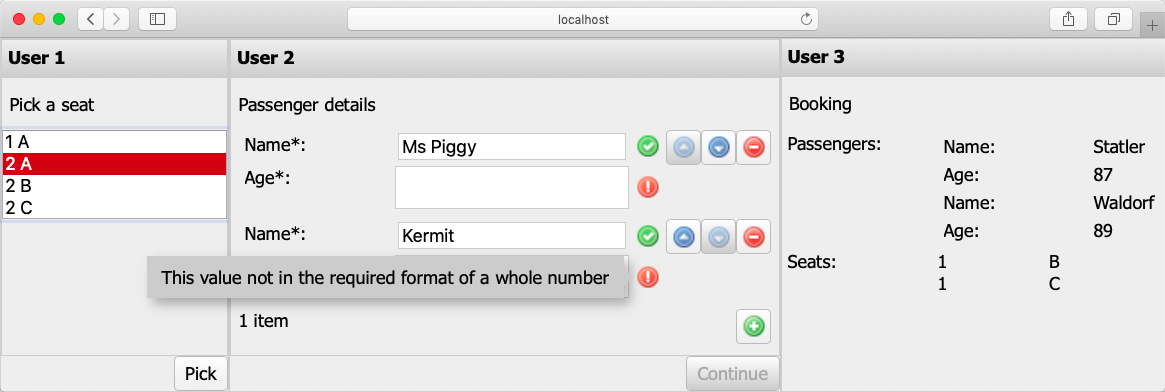
\includegraphics[width=\columnwidth]{figures/flight-booking.png}
  \caption{
    Running web application of the flight booking example using a translation to \ITASKS,
    a \TOP implementation.
    It shows three users booking a flight simultaneously.
    The first user entered name and age and continued to picking seats.
    The second is entering details of two passengers.
    The ages are not filled in, and therefore the \TS{Continue} button is disabled.
    The third user finished a booking.
    Note the first user can't pick seats \smallcaps{1b} and \smallcaps{1c} any more.
    Also, the message bubble shows it is only allowed to enter an integer in the \TS{age} field.
  }
  \label{fig:flight-booking}
\end{figure}



%% Acknowledgments
% \begin{acks}                            %% acks environment is optional
%                                         %% contents suppressed with 'anonymous'
%   %% Commands \grantsponsor{<sponsorID>}{<name>}{<url>} and
%   %% \grantnum[<url>]{<sponsorID>}{<number>} should be used to
%   %% acknowledge financial support and will be used by metadata
%   %% extraction tools.
%   \small
%   % !TEX root=../icfp2019.tex

The authors are grateful to Johan Jeuring, Sjaak Smetsers, and Andreas Vinter-Hviid for fruitful discussions,
and Rinus Plasmeijer, Peter Achten and Pieter Koopman for proofreading.

This research is supported by the Dutch Technology Foundation STW, which is part
of the Netherlands Organisation for Scientific Research (NWO), and which is
partly funded by the Ministry of Economic Affairs.

% \end{acks}


%% Bibliography
\bibliography{bibliography}


% \pagebreak
% %% Appendix
%
% % !TEX root=../pldi2019.tex

\appendix
\section{Appendix}

  \subsection{Rules}

    \begin{mathpar}
      \boxed{\RelationT} \\
      \userule{T-Abs}\qquad
      \userule{T-Var}\\
      \userule{T-If}\\
      \userule{T-App}\qquad
      \userule{T-Ref}\\
      \userule{T-Deref}\qquad
      \userule{T-Loc}\\
      \userule{T-Assign}\qquad
      \userule{T-Pair}\\
    \end{mathpar}

    \begin{mathpar}
      \boxed{\RelationE} \\
      \userule{E-Value}\\
      \userule{E-App}\\
      \userule{E-IfTrue}\quad
      \userule{E-IfFalse}\\
      \userule{E-Pair}\quad
      \userule{E-Ref}\\
      \userule{E-Deref}\quad
      \userule{E-Assign}\\
      \userule{E-Sequence}\\
    \end{mathpar}

  \subsection{Proofs}

  \subsubsection{Theorem~\ref{thmpreseval}}
\begin{proof}
  We prove Theorem~\ref{thmpreseval} by induction on $e$:\\

  \noindent\textbf{Case} $e=\lambda x:\tau.e, e_1 e_2, x, c, l, e_1 \star e_2,
      \If{e_1}{e_2}{e_3},$\\
      $\tuple{e_1, e_2},\unit,\Ref e,!e,e_1 := e_2,e_1; e_2$ preservation has
      been proven for these cases by \todo{insert cite}\\

  \noindent\textbf{Case} $\userule{E-Edit}$
      Given that $\Gamma,\Sigma\infers\Edit e:\Task \tau$ and $\Sigma\infers s$, T-Edit gives us that
      $\Gamma,\Sigma\infers e:\tau$. The induction hypothesis gives us that
      $e,s\evaluate v,s'$ also preserves, and thus $\Gamma,\Sigma\infers v:\tau$
      and $\Sigma\infers s'$. Therefore $\Gamma,\Sigma\infers\Edit v:\Task\tau$.\\

  \noindent\textbf{Case} $\userule{E-Fill}$
      Evaluation does not alter $e$ and $s$, therefore this case holds tivially.\\

  \noindent\textbf{Case} $\userule{E-Update}$
      Given that $\Gamma,\Sigma\infers \Edit e:\Task \tau$ and
      $\Sigma\infers s$, T-Update gives us that $\Gamma,\Sigma\infers e:\Ref \tau$.
      The induction hypothesis gives us that $e,s\evaluate l,s'$ also preserves,
      and thus $\Gamma,\Sigma\infers l:\Ref\tau$ and $\Sigma\infers s'$.
      Therefore $\Gamma,\Sigma\infers\Update l:\Task\tau$\\

  \noindent\textbf{Case} $\userule{E-Fail}$
      Evaluation does not alter $e$ and $s$, therefore this case holds tivially.\\

  \noindent\textbf{Case} $\userule{E-Then}$
      Given that $\Gamma,\Sigma\infers e_1\Then e_2:\Task \tau$ and $\Sigma\infers s$, T-Then gives us that $\Gamma,\Sigma\infers e_1:\Task\tau_1$
      and $\Gamma,\Sigma\infers e_2:\tau_1 \to \Task \tau$. By the induction hypothesis, we know that
      $e_1,s\evaluate t_1,s'$ preserves and thus $\Gamma,\Sigma\infers t_1:\Task\tau_1$ and $\Sigma\infers s'$. Therefore
      $\Gamma,\Sigma\infers t_1\Then e_2:\Task\tau$.\\

  \noindent\textbf{Case} $\userule{E-Next}$
      Given that $\Gamma,\Sigma\infers e_1\Next e_2:\Task \tau$ and $\Sigma\infers s$, T-Then gives us that $\Gamma,\Sigma\infers e_1:\Task\tau_1$
      and $\Gamma,\Sigma\infers e_2:\tau_1 \to \Task \tau$. By the induction hypothesis, we know that
      $e_1,s\evaluate t_1,s'$ preserves and thus $\Gamma,\Sigma\infers t_1:\Task\tau_1$ and $\Sigma\infers s'$. Therefore
      $\Gamma,\Sigma\infers t_1\Next e_2:\Task\tau$.\\

  \noindent\textbf{Case} $\userule{E-And}$
      Given that $\Gamma,\Sigma\infers e_1\And e_2:\Task(\tau_1\times\tau_2)$ and $\Sigma\infers s$, T-And gives us that
      $\Gamma,\Sigma\infers e_1:\Task\tau_1$ and $\Gamma,\Sigma\infers e_2:\Task\tau_2$. By the induction hypothesis, we
      know that both $e_1,s\evaluate t_1,s'$ and $e_2,s'\evaluate t_2,s''$ preserve and thus
      $\Gamma,\Sigma\infers t_1:\Task\tau_1$, $\Sigma\infers s'$, $\Gamma,\Sigma\infers t_2:\Task\tau_2$ and $\Sigma\infers s''$. Therfore
      $\Gamma,\Sigma\infers t_1\And t_2:\Task(\tau_1\times\tau_2)$\\

  \noindent\textbf{Case} $\userule{E-Or}$
      Given that $\Gamma,\Sigma\infers e_1\Or e_2:\Task\tau$ and $\Sigma\infers s$, T-Or gives us that $\Gamma,\Sigma\infers e_1:\Task\tau$ and
      $\Gamma,\Sigma\infers e_2:\Task\tau$. By the induction hypothesis, we have that both
      $e_1,s\evaluate t_1,s'$ and $e_2,s'\evaluate t_2,s''$ preserve and thus $\Gamma,\Sigma\infers t_1:\Task\tau$, $\Sigma\infers s'$,
      $\Gamma,\Sigma\infers t_2:\Task\tau$ and $\Sigma\infers s''$. Therefore $\Gamma,\Sigma\infers t_1\Or t_2:\Task\tau$.\\

  \noindent\textbf{Case} $\userule{E-Xor}$
      Evaluation does not alter $e$ and $s$, therefore this case holds tivially.\\

  \noindent\textbf{Case} $\userule{E-Appoint}$
      Given that $\Gamma,\Sigma\infers u \At e:\Task\tau$ and $\Sigma\infers s$, the induction hypothesis gives us that $e,s\evaluate t,s'$ also preserves, and therefore by T-Appoint $\Gamma,\Sigma\infers u \At t:\Task\tau$.
\end{proof}



\subsubsection{Lemma~\ref{lemmavaluepreserves}}
\begin{proof}
  We prove Lemma~\ref{lemmavaluepreserves} by induction over $e$.\\

  \noindent\textbf{Case} $\Value{(\Edit v,s)}=v$ By T-Edit, if $\Gamma,\Sigma\infers \Edit v:\Task\tau$, then $\Gamma,\Sigma\infers v:\tau$.\\

  \noindent\textbf{Case} $\Value{(\Enter \tau,s)}=\bot$ Since this case does not lead to a value, the lemma holds trivially.\\

  \noindent\textbf{Case} $\Value{(\Update l,s)}=s(l)$ Given that $\Gamma,\Sigma\infers\Update l:\Task \tau$ and $\Sigma\infers s$, we know that $\Gamma,\Sigma\infers s(l):\tau$.\\

  \noindent\textbf{Case} $\Value{(\Fail,s)}=\bot$ Since this case does not lead to a value, the lemma holds trivially.\\

  \noindent\textbf{Case} $\Value{(t_1\Then e_2,s)}=\bot$ Since this case does not lead to a value, the lemma holds trivially.\\

  \noindent\textbf{Case} $\Value{(t_2\Next e_2,s)}=\bot$ Since this case does not lead to a value, the lemma holds trivially.\\

  \noindent\textbf{Case} $\Value{(t_1\And t_2,s)}=\tuple{v_1, v_2}$ given that $\Value{(t_1,s)}=v_1\wedge\Value{(t_2,s)}=v_2$\\ By T-And we have that $\Gamma,\Sigma\infers t_1\And t_2:\Task(\tau_1\times\tau_2)$ and $\Gamma,\Sigma\infers t_1:\tau_1$ and $\Gamma,\Sigma\infers t_2:\tau_2$. By the induction hypothesis, $ \Value{(t_1,s)}=v_1$ and $\Value{(t_2,s)}=v_2$ preserve, and thus $\Gamma,\Sigma\infers v_1:\tau_1$ and $\Gamma,\Sigma\infers v_2:\tau_2$. This gives us that $\Gamma,\Sigma\infers \tuple{v_1, v_2}:\Task(\tau_1\times\tau_2)$ \\

  \noindent\textbf{Case} $\Value{(t_1\And t_2,s)}=\bot$ given that $\neg(\Value{(t_1,s)}=v_1\wedge\Value{(t_2,s)}=v_2)$\\ Since this case does not lead to a value, the lemma holds trivially.\\

  \noindent\textbf{Case} $\Value{(t_1\Or t_2,s)}=v_1$ given that $\Value{(t_1,s)}=v_1$\\ By T-Or we have that $\Gamma,\Sigma\infers t_1\Or t_2:\Task\tau$, and $\Gamma,\Sigma\infers t_1:\Task\tau$ and $\Gamma,\Sigma\infers t_2:\Task\tau$. By the induction hypothesis, we have that $\Gamma,\Sigma\infers v_1:\tau$.\\

  \noindent\textbf{Case} $\Value{(t_1\Or t_2,s)}=v_2$ given that $\Value{(t_1,s)}=\bot\wedge\Value{(t_2,s)}=v_2$\\ By T-Or we have that $\Gamma,\Sigma\infers t_1\Or t_2:\Task\tau$, and $\Gamma,\Sigma\infers t_1:\Task\tau$ and $\Gamma,\Sigma\infers t_2:\Task\tau$. By the induction hypothesis, we have that $\Gamma,\Sigma\infers v_2:\tau$.\\

  \noindent\textbf{Case} $\Value{(t_1\Or t_2,s)}=\bot$ given that $\Value{(t_1,s)}=\bot\wedge\Value{(t_2,s)}=\bot$\\ Since this case does not lead to a value, the lemma holds trivially.\\

  \noindent\textbf{Case} $\Value{(t_1\Xor t_2,s)}=\bot$ Since this case does not lead to a value, the lemma holds trivially.\\
\end{proof}



\subsubsection{Theorem~\ref{thmpresnorm}}
\begin{proof}
  We prove Theorem~\ref{thmpresnorm} by induction on $e$:\\

  \noindent\textbf{Case} $\userule{N-Fail}$ Since this case does not alter the
  expression, the theorem holds trivially.\\

  \noindent\textbf{Case} $\userule{N-Xor}$ Since this case does not alter the
  expression, the theorem holds trivially.\\

  \noindent\textbf{Case} $\userule{N-Update}$ Since this case does not alter
  the expression, the theorem holds trivially.\\

  \noindent\textbf{Case} $\userule{N-Fill}$ Since this case does not alter the
  expression, the theorem holds trivially.\\

  \noindent\textbf{Case} $\userule{N-Edit}$ Since this case does not alter the
  expression, the theorem holds trivially.\\

  \noindent\textbf{Case} $\userule{N-And}$ Given that $t_1\And t_2:\Task(\tau_1\times\tau_2)$, by T-And we have $t_1:\tau_1$ and $t_2:\tau_2$. By the induction hypothesis, we also have $t_1':\tau_1$ and $t_2':\tau_2$. This gives us that $t_1'\And t_2':\Task(\tau_1\times\tau_2)$.\\

  \noindent\textbf{Case} $\userule{N-Next}$ Given that $e_1\Next e_2:\Task \tau$, T-Then gives us that $t_1:\Task\tau_1$
  and $e_2:\tau_1 \to \Task \tau$. By the induction hypothesis, we know that
  $t_1\normalise t_1'$ preserves and thus $t_1':\Task\tau_1$. Therefore
  $t_1'\Next e_2:\Task\tau$.\\\\

  \noindent\textbf{Case} $\userule{N-OrLeft}$ Given that $t_1\Or t_2:\Task\tau$,
  by T-Or we have $t_1:\Task\tau$. By the induction hypothesis, we know that
  $t_1\normalise t_1'$ preserves and thus $t_1':\Task\tau$.\\

  \noindent\textbf{Case} $\userule{N-OrRight}$ Given that $t_1\Or t_2:\Task\tau$,
  by T-Or we have $t_2:\Task\tau$. By the induction hypothesis, we know that
  $t_2\normalise t_2'$ preserves and thus $t_2':\Task\tau$. \todo{there might be
  more to be said here. t1 obviously can to stuff too, but we don't say anyting about this.}\\

  \noindent\textbf{Case} $\userule{N-OrNone}$ Given that $t_1\Or t_2:\Task\tau$,
  by T-Or we have $t_1:\Task\tau$ and $t_2:\Task\tau$. By the induction hypothesis,
  we know that $t_1\normalise t_1'$ and $t_2\normalise t_2'$ preserve, and thus
  $t_1'\Or t_2':\Task\tau$.\\

  \noindent\textbf{Case} $\userule{N-ThenStay}$ Given that $t_1\Then e_2:\Task\tau$,
  by T-Then we have $t_1:\Task\tau_1$ and $e_2:\tau_1\to\Task\tau$. By the induction
  hypothesis, we know that $t_1\normalise t_1'$ preserves, and thus $t_1'\Then e_2:\Task\tau$.\\

  \noindent\textbf{Case} $\userule{N-ThenFail}$ Given that $t_1\Then e_2:\Task\tau$,
  by T-Then we have $t_1:\Task\tau_1$ and $e_2:\tau_1\to\Task\tau$. By the induction
  hypothesis, we know that $t_1\normalise t_1'$ preserves, and thus $t_1'\Then e_2:\Task\tau$.\\

  \noindent\textbf{Case} $\userule{N-ThenCont}$Given that $t_1\Then e_2:\Task\tau$,
  by T-Then we have $t_1:\Task\tau_1$ and $e_2:\tau_1\to\Task\tau$. By the induction
  hypothesis, we know that $t_1\normalise t_1'$ preserves. By
  Lemma~\ref{lemmavaluepreserves}, we know that $\Value{(t_1')}=v_1$ preserves.
  By Theorem~\ref{thmpreseval} we know that $e_2 v_1\evaluate t_2$ preserves. And
  finally by the induction hypothesis, we know that $t_2\normalise t_2'$ preserves.
  Therefore $t_2':\Task\tau$.\\

\end{proof}


\subsubsection{Theorem~\ref{thmpreshandle}}

We require the following Lemma for this proof.

\begin{lemma}
  Given that $\Sigma\infers s$, $\Sigma(l)=\tau$ and $\Gamma,\Sigma\infers v:\tau$, it holds that $\Sigma\infers s[l\mapsto v]$
  \label{lemmasigmaconsistent}
\end{lemma}
This lemma follows immediately from definition.

\begin{proof}
  We prove Theorem~\ref{thmpreshandle} by induction on $e$:

  \noindent\textbf{Case} $\userule{H-Change}$ Given that $\Gamma,\Sigma\infers\Edit v:\Task\tau$ and $\Sigma\infers s$, the H-Change rule additionally gives us that $v,v':\tau$. Therefore by T-Edit we have that $\Gamma,\Sigma\infers\Edit v':\Task\tau$\\

  \noindent\textbf{Case} $\userule{H-Empty}$ Given that $\Gamma,\Sigma\infers\Edit v:\Task\beta$ and $\Sigma\infers s$, the H-Empty rule additionally gives us that $v:\tau$. Then by T-Fill we have $\Gamma,\Sigma\infers\Enter \tau:\Task\tau$ \\

  \noindent\textbf{Case} $\userule{H-Fill}$ Given that $\Gamma,\Sigma\infers\Enter\tau$ and $\Sigma\infers s$, the H-Fill rule additionally gives us that $v':\tau$. Then by T-Fill we have $\Gamma,\Sigma\infers \Edit v':\Task\tau$.\\

  \noindent\textbf{Case} $\userule{H-Update}$ Given that $\Gamma,\Sigma\infers\Update l:\Task\tau$ and $\Sigma\infers s$. This gives us that $\Sigma(l)=\tau$, and we additionally obtain $s(l),v':\tau$ by H-Update. By application of Lemma~\ref{lemmasigmaconsistent} this case holds.\\

  \noindent\textbf{Case} $\userule{H-PickLeft}$ Given that $\Gamma,\Sigma\infers t_1\Xor t_2:\Task\tau$ and $\Sigma\infers s$, then by T-Xor we have $\Gamma,\Sigma\infers t_1:\Task \tau$.\\

  \noindent\textbf{Case} $\userule{H-PickRight}$ Given that $\Gamma,\Sigma\infers t_1\Xor t_2:\Task\tau$ and $\Sigma\infers s$, then by T-Xor we have $\Gamma,\Sigma\infers t_2:\Task \tau$. \\

  \noindent\textbf{Case} $\userule{H-Next}$ Given that $\Gamma,\Sigma\infers t_1\Next e_2 :\Task\tau$ and $\Sigma\infers s$. Then by T-Next, we have $\Gamma,\Sigma\infers t_1:\Task\tau_1$ and $\Gamma,\Sigma\infers e_2:\tau_1\to\Task\tau$. Then by T-Then we obtain $\Gamma,\Sigma\infers t_1\Then e_2:\Task\tau$.\\

  \noindent\textbf{Case} $\userule{H-PassThen}$ Given that $\Gamma,\Sigma\infers t_1\Then e_2:\Task\tau$ and $\Sigma\infers s$, T-Then gives us that $\Gamma,\Sigma\infers t_1:\Task\tau_1$ and $\Gamma,\Sigma\infers e_2:\tau_1\to\Task\tau$. By the induction hypothesis, we know that $t_1,s\handle{i}t_1',s'$ also preserves and thus $\Gamma,\Sigma\infers t_1':\Task\tau_1$ and $\Gamma,Sigma\infers s'$. By T-Then we now obtain that $\Gamma,\Sigma\infers t_1'\Then e_2:\Task\tau$. \\

  \noindent\textbf{Case} $\userule{H-PassNext}$ Given that $\Gamma,\Sigma\infers t_1\Next e_2:\Task\tau$ and $\Sigma\infers s$, T-Next gives us that $\Gamma,\Sigma\infers t_1:\Task\tau_1$ and $\Gamma,\Sigma\infers e_2:\tau_1\to\Task\tau$. By the induction hypothesis, we know that $t_1,s\handle{i}t_1',s'$ also preserves and thus $\Gamma,\Sigma\infers t_1':\Task\tau_1$ and $\Gamma,Sigma\infers s'$. By T-Next we now obtain that $\Gamma,\Sigma\infers t_1'\Next e_2:\Task\tau$. \\

  \noindent\textbf{Case} $\userule{H-FirstAnd}$ Given that $\Gamma,\Sigma\infers t_1\And t_2:\Task(\tau_1\times\tau_2)$ and $\Sigma\infers s$, T-And gives us that $\Gamma,\Sigma\infers t_1:\Task\tau_1$ and $\Gamma,\Sigma\infers t_2:\Task\tau_2$. By the induction hypothesis, we know that $t_1,s\handle{i}t_1',s'$ also preserves and thus $\Gamma,\Sigma\infers t_1':\Task\tau_1$ and $\Sigma\infers s'$. Therefore by T-Next we obtain $\Gamma,\Sigma\infers t_1'\And t_2:\Task(\tau_1\times\tau_2)$.\\

  \noindent\textbf{Case} $\userule{H-SecondAnd}$ Given that $\Gamma,\Sigma\infers t_1\And t_2:\Task(\tau_1\times\tau_2)$ and $\Sigma\infers s$, T-And gives us that $\Gamma,\Sigma\infers t_1:\Task\tau_1$ and $\Gamma,\Sigma\infers t_2:\Task\tau_2$. By the induction hypothesis, we know that $t_2,s\handle{i}t_2',s'$ also preserves and thus $\Gamma,\Sigma\infers t_2':\Task\tau_2$ and $\Sigma\infers s'$. Therefore by T-Next we obtain $\Gamma,\Sigma\infers t_1\And t_2':\Task(\tau_1\times\tau_2)$.\\

  \noindent\textbf{Case} $\userule{H-FirstOr}$ Given that $\Gamma,\Sigma\infers t_1\Or t_2:\Task\tau$ and $\Sigma\infers s$, T-Or gives us that $\Gamma,\Sigma\infers t_1:\Task\tau$ and $\Gamma,\Sigma\infers t_2:\Task\tau$. By the induction hypothesis we know that $t_1,s\handle{i}t_1',s'$ also preserves, and therefore $\Gamma,\Sigma\infers t_1':\Task\tau$ and $\Sigma\infers s'$. By T-Or we now obtain $\Gamma,\Sigma\infers t_1'\Or t_2:\Task\tau$.\\

  \noindent\textbf{Case} $\userule{H-SecondOr}$ Given that $\Gamma,\Sigma\infers t_1\Or t_2:\Task\tau$ and $\Sigma\infers s$, T-Or gives us that $\Gamma,\Sigma\infers t_1:\Task\tau$ and $\Gamma,\Sigma\infers t_2:\Task\tau$. By the induction hypothesis we know that $t_2,s\handle{i}t_2',s'$ also preserves, and therefore $\Gamma,\Sigma\infers t_2':\Task\tau$ and $\Sigma\infers s'$. By T-Or we now obtain $\Gamma,\Sigma\infers t_1\Or t_2':\Task\tau$.
\end{proof}

% \subsubsection{Theorem~\ref{thmprogressnorm}}
%
% \begin{proof} We prove this Theorem by induction on $e$.\\
%
%   \noindent\textbf{Case} $\userule{N-Edit}$ Given that $\Gamma,\Sigma\infers \Edit v : \Task \tau$, let $e''=\Edit v'$, $s''=s$ and $i=v':\tau$. Then H-Edit gives $\Edit v,s\handle{v'}\Edit v',s$. \\
%
%
%   \noindent\textbf{Case} $\userule{N-Fill}$ Given that $\Gamma,\Sigma\infers \Enter \tau : \Task \tau$, let $e''=\Edit v$, $s''=s$ and $i=v:\tau$. Then H-Fill gives $\Enter \tau,s\handle{v}\Edit v,s$. \\
%
%   \noindent\textbf{Case} $\userule{N-Update}$ Given that $\Gamma,\Sigma\infers \Update l : \Task \tau$, let $e''=\Update l$, $s''=s[l\mapsto v]$ and $i=v:\tau$. Then H-Update gives $\Update l ,s\handle{v}\Update l,s[l\mapsto v]$. \\
%
%   \noindent\textbf{Case} $\userule{N-Fail}$ Since $\Failing(\Fail)=\True$, the theorem holds in this case. \\
%
%   \noindent\textbf{Case} $\userule{N-Xor}$ \todo{Here we have an issue with the defintion of $\Failing$ and the sideconditions of external choice. These definitions should concur, so we can finish the proof, but $\Failing$ is a static property}\\
%
%   \noindent\textbf{Case} $\userule{N-Eval}$ By induction hypothesis we have that there exists an $e'''$, $s'''$ and $i$ such that $e'',s''\handle{i}e''',s'''$.\\
%
%   \noindent\textbf{Case} $\userule{N-ThenStay}$ By the induction hyposthesis we have that there exists an $e''$, $s''$ and $i$ such that $t_1',s'\handle{i}e'',s''$. Then by H-Pass, we know that we can apply the same $i$ to obtain $t_1\Then e_2,s'\handle{i} e''\Then e,s''$.\\
%
%   \noindent\textbf{Case} $\userule{N-ThenFail}$ By the induction hyposthesis we have that there exists an $e''$, $s''$ and $i$ such that $t_1',s'\handle{i}e'',s''$. Then by H-Pass, we know that we can apply the same $i$ to obtain $t_1\Then e_2,s'\handle{i} e''\Then e,s''$.\\
%
%   \noindent\textbf{Case} $\userule{N-ThenCont}$ By the induction hypothesis, we have that there exists an $e''$, $s''''$ and $i$ such that $t_2',s''\handle{i}e'',s''''$.\\
%
%   \noindent\textbf{Case} $\userule{N-OrLeft}$ By the induction hypothesis, we have that there exists an $e''$, $s'$ and $i$ such that $t_1',s\handle{i}e'',s''$.\\
%
%   \noindent\textbf{Case} $\userule{N-OrRight}$ By the induction hypothesis, we have that there exists an $e''$, $s'$ and $i$ such that $t_2',s\handle{i}e'',s''$.\\
%
%   \noindent\textbf{Case} $\userule{N-OrNone}$ \todo{   }\\
%
%   \noindent\textbf{Case} $\userule{N-Next}$ By the induction hypothesis, we have that there exists an $e''$, $s'$ and $i$ such that $t_1',s'\handle{i}e'',s''$. Then by the H-PassNext rule, we know that we can apply the same $i$ to obtain $t_1'\Next e_2,s'\handle{i}e'',s''$.\\
%
%   \noindent\textbf{Case} $\userule{N-And}$ By the induction hypothesis, we have that there exists an $e''$, $s'$ and $i$ such that $t_1',s'\handle{i}e'',s''$. Then by the H-FirstOr rule, we know that we can apply $\First i$ to obtain $t_1'\And t_2',s'\handle{\First i} t_1''\And t_2',s''$
%
% \end{proof}


\subsubsection{Theorem~\ref{thmnormisbigstep}}

\begin{proof}
  We prove Theorem~\ref{thmpresnorm} by induction on $e$:\\

  \noindent\textbf{Case} $\userule{N-Done}$\\

  \noindent\textbf{Case} $\userule{N-Stride}$\\

  \noindent\textbf{Case} $\userule{N-Fail}$ \\

  \noindent\textbf{Case} $\userule{N-Xor}$ \\

  \noindent\textbf{Case} $\userule{N-Update}$ \\

  \noindent\textbf{Case} $\userule{N-Fill}$ \\

  \noindent\textbf{Case} $\userule{N-Edit}$ \\

  \noindent\textbf{Case} $\userule{N-And}$ \\

  \noindent\textbf{Case} $\userule{N-Next}$ \\

  \noindent\textbf{Case} $\userule{N-OrLeft}$ \\

  \noindent\textbf{Case} $\userule{N-OrRight}$ \\

  \noindent\textbf{Case} $\userule{N-OrNone}$\\

  \noindent\textbf{Case} $\userule{N-ThenStay}$\\

  \noindent\textbf{Case} $\userule{N-ThenFail}$\\

  \noindent\textbf{Case} $\userule{N-ThenCont}$\\

  \noindent\textbf{Case} $\userule{N-Assign}$

\end{proof}

\subsubsection{Theorem~\ref{thmfailing}}

We prove Theorem~\ref{thmfailing} by induction on $e'$.

\begin{proof}

  \noindent\textbf{Case} $e = \Fail$ $\Failing(\Fail)=\True$, and there is no handling rule that applies to fail.\\

  \noindent\textbf{Case} $e = \Edit v$ Given that $\Gamma,\Sigma\infers\Edit v:\Task\tau$, $\Failing(\Edit v)=\False$, and there exists an input $i$, namely $v':\tau$.\\

  \noindent\textbf{Case} $e = \Enter \tau$ $\Failing(\Enter \tau)=\False$, and there exists an in put i, namely $v:\tau$.\\

  \noindent\textbf{Case} $e = \Update l$ Given that $\Gamma,\Sigma\infers\Update l:\Task\tau$, $\Failing(\Update l)=\False$, and there exists an input $i$, namely $v:\tau$.\\

  \noindent\textbf{Case} $e = t_1\Then e_2$ $\Failing(t_1\Then e_2)=\Failing(t_1)$. If there exitsts an $i$ for $t_1$, then this $i$ also applies to $t_1\Then e_2$. This case therefore holds by the induction hypothesis.\\

  \noindent\textbf{Case} $e = t_1\Next e_2$ $\Failing(t_1\Next e_2)=\Failing(t_1)$. If there exitsts an $i$ for $t_1$, then this $i$ also applies to $t_1\Next e_2$. This case therefore holds by the induction hypothesis.\\

  \noindent\textbf{Case} $e = e_1\Xor e_2$ We normalise the two expressions first, $e_1,s\normalise t_1,s'$, $e_2,s\normalise t_2,s'$ and we can then be in two situations. One, we can have that $\Failing(t_1,s')$ and $\Failing(t_2,s')$ are both true. If that is so, then by definiton, we have both $\Failing(e_1\Xor e_2,s)$ and no rule of the hanlding semantics applies, and therefore there exists no input for this case.\\
                                           Or we are in the situation where one or both of the two sub expressions does not fail. In that case, we know that $\Failing(e_1\Xor e_2,s)$ does not hold, and that at least one of the handling rules applies. Therefore, there must be an input $i$, namely $\Left$, $\Right$ or both.

  \noindent\textbf{Case} $e = t_1\And t_2$ We can again find ourselfs in one of two situations. In the first case, both sub expressions fail, $\Failing(t_1,s)$ and $\Failing(t_2,s)$. In that case, we know that $\Failing(t_1\And t_2,s)$ also fails by definition. By the induction hypothesis, we know that for both $t_1$ and $t_2$ there is no input that can be handled. Since the only two rules for $\And$ that handle input just pass this input on to one of the two expressions, we know that indeed no $i$ applies.\\
                                           In the case that one or both sub expressions do not fail, then by definition $t_1\And t_2$ not failing under $s$. Again by induction hypothesis, we know that for one or both of the expressions, there exits an $i$ that can be handled. Then by H-FirstAnd and H-SecondAnd, we know that we can pass this $i$, by prefixing it with either $\First$ or $\Second$.\\

  \noindent\textbf{Case} $e = t_1\Or t_2$We can again find ourselfs in one of two situations. In the first case, both sub expressions fail, $\Failing(t_1,s)$ and $\Failing(t_2,s)$. In that case, we know that $\Failing(t_1\Or t_2,s)$ also fails by definition. By the induction hypothesis, we know that for both $t_1$ and $t_2$ there is no input that can be handled. Since the only two rules for $\Or$ that handle input just pass this input on to one of the two expressions, we know that indeed no $i$ applies.\\
                                           In the case that one or both sub expressions do not fail, then by definition $t_1\Or t_2$ not failing under $s$. Again by induction hypothesis, we know that for one or both of the expressions, there exits an $i$ that can be handled. Then by H-FirstOr and H-SecondOr, we know that we can pass this $i$, by prefixing it with either $\First$ or $\Second$.\\

  \noindent\textbf{Case} $e = u \At t$ This case follows directly from applying the induction hypothesis, since $\Failing(u \At t,s)=\Failing(t,s)$ and any input that applies to $t$ also applies to $u \At t$.\\
\end{proof}

\subsubsection{Theorem~\ref{thmsafetyi1}}

\begin{proof}
  \noindent\textbf{Case} $\Edit v:\Task\tau$ By definition, $\Inputs{(\Edit v)}=\{v',\Empty\}$. For $i=v'$, we have that $\userule{H-Change}$ handles the input, and for $i=\Empty$, we have $\userule{H-Empty}$.\\

  \noindent\textbf{Case} $\Enter \tau$ By definition, $\Inputs{(\Enter \tau)}=\{v':\tau\}$. For $i=v'$, we have that $\userule{H-Fill}$ handles the input.\\

  \noindent\textbf{Case} $\Update l:\Task\tau$ By definition, $\Inputs{(\Update\tau)}=\{v'\}$. For $i=v'$, we have that $\userule{H-Update}$ handles the input.\\

  \noindent\textbf{Case} $\Fail$ By definition, $\Inputs{(\Fail)}=\{\}$. The theorem holds trivially.\\

  \noindent\textbf{Case} $t_1\Then e_2$ By definition, $\Inputs{(t_1\Then e_2)}=\Inputs{(t_1)}$. By the induction hypothesis, we have that $i\in\Inputs{(t_1)}$, then $t_1\handle{i}t_1'$. Therefore, we also have $\userule{H-PassThen}$.\\

  \noindent\textbf{Case} $t_1\Next e_2$ By definiton, $\Inputs(t_1 \Next e_2) = \Inputs(t_1) \cup \set{\Continue\mid \Value{(t_1)}\neq \bot \wedge \neg\Failing{(e_2 \Value{(t_1)}\normalise)}}$. If $i=\Continue$, then we know that $\Value{(t_1)}\neq \bot \wedge \neg\Failing{(e_2 \Value{(t_1)}\normalise)}$ holds, and therefore H-Next applies. Otherwise, we have by induction hypothesis that $i\in\Inputs{(t_1)}$, then $t_1\handle{i}t_1'$. Therefore, we also have $\userule{H-PassNext}$.\\

  \noindent\textbf{Case} $t_1\And t_2$ By definiiton, $\Inputs(t_1\And t_2) = \set{\First\ i \mid i \in \Inputs(t_1)} \cup \set{\Second\ i \mid i \in \Inputs(t_2)}$. By the induction hypothesis, we have both that if $i\in\Inputs(t_1)$ then $t_1\handle{i}t_1'$ and that if $i\in\Inputs(t_2)$ then $t_2\handle{i}t_2'$. Therefore, if $i\in\Inputs(t_1\And t_2)$, then either $\userule{H-FirstAnd}$ or $\userule{H-SecondAnd}$.\\

  \noindent\textbf{Case} $t_1\Or t_2$ By definition, $\Inputs(t_1\Or t_2) = \set{\First\ i \mid i \in \Inputs(t_1)} \cup \set{\Second\ i \mid i \in \Inputs(t_2)}$. By the induction hypothesis, we have both that if $i\in\Inputs(t_1)$ then $t_1\handle{i}t_1'$ and that if $i\in\Inputs(t_2)$ then $t_2\handle{i}t_2'$. Therefore, if $i\in\Inputs(t_1\Or t_2)$, then either $\userule{H-FirstOr}$ or $\userule{H-SecondOr}$.\\

  \noindent\textbf{Case} $t_1\Xor t_2$ By definition, $\Inputs(t_1\Xor t_2) = \set{\Pick \Left, \Pick \Right}$. In case $i=\Pick\Left$, H-PickLeft applies, in case $i=\Pick\Right$, H-PickRight applies.

\end{proof}

\subsubsection{Theorem~\ref{thmsafetyi2}}
\begin{proof}
  \noindent\textbf{Case} $e=\Edit v:\Task\tau, i= v':\tau$\\
  \noindent\textbf{Case} $e=\Edit v:\Task\tau, i= \Empty$\\
  \noindent\textbf{Case} $e=\Enter \tau, i= v':\tau$\\
  \noindent\textbf{Case} $e=\Update l:\Task\tau, i= v':\tau$\\
  \noindent\textbf{Case} $e=t_1\Or t_2 , i= \Pick\Left r $\\
  \noindent\textbf{Case} $e=t_1\Or t_2 , i= \Pick\Right r $\\
  \noindent\textbf{Case} $e=t, i= \Pick\Here $\\
  \noindent\textbf{Case} $e=t_1\Next e_2 , i= \Continue $\\
  \noindent\textbf{Case} $e=t_1\Then e_2 , i$\\
  \noindent\textbf{Case} $e=t_1\Next e_2 , i\neq\Continue$\\
  \noindent\textbf{Case} $e=t_1\And t_2 , i=\First i$\\
  \noindent\textbf{Case} $e=t_1\And t_2 , i=\Second i$\\
  \noindent\textbf{Case} $e=t_1\Or t_2 , i=\First i$\\
  \noindent\textbf{Case} $e=t_1\Or t_2 , i=\Second i$\\
\end{proof}



\end{document}
